\section{The least squares problem}

The ordinary linear least squares problem, simply stated, is
\[
  \operatorname{minimize}_x \|Ax-b\|_2^2
\]
where $A \in \bbR^{m \times n}$ with $m > n$.
Unless otherwise stated, we will assume that undecorated norms
refer to the two-norm for this part of the course.

\subsection{The normal equations}

\begin{figure}
  \begin{center}
  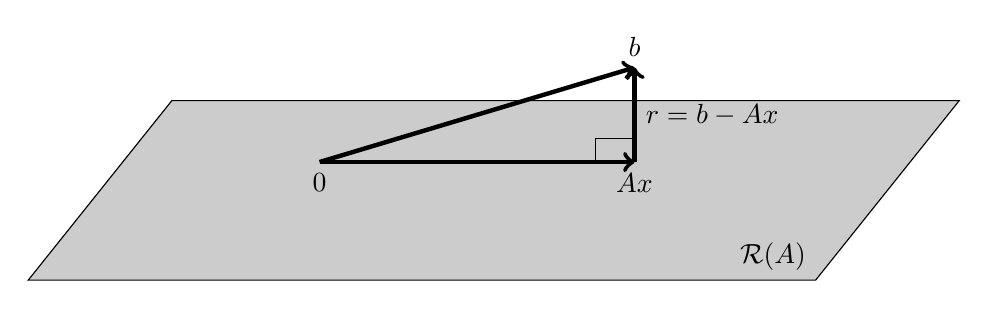
\begin{tikzpicture}
    \begin{scope}[xslant=0.8,xscale=5,yscale=3]
      \draw[fill=black!20] (-0.5,-0.5) rectangle (1.5,0.26);
      \draw[ultra thick,->]
        (0,0) node[below] {$0$} --
        (0.8,0) node[below] {$Ax$};
      \node[above left] at (1.5,-0.5) {$\mathcal{R}(A)$};
    \end{scope}
    \begin{scope}[xscale=5,yscale=3]
    \draw[ultra thick,->]
      (0,0) -- (0.8,0.4) node[above] {$b$};
    \draw[ultra thick,->]
      (0.8,0) -- (0.8,0.4) node[midway,right] {$r=b-Ax$};
    \draw (0.7,0) -- (0.7,0.1) -- (0.8,0.1);
    \end{scope}
  \end{tikzpicture}
  \end{center}
  \caption{Picture of a linear least squares problem.  The vector $Ax$
           is the closest vector in $\mathcal{R}(A)$ to a target
           vector $b$ in the Euclidean norm.  Consequently, the
           residual $r = b-Ax$ is normal (orthogonal) to
           $\mathcal{R}(A)$.}
  \label{fig1}
\end{figure}

The quantity
$r = Ax-b$ is the least squares residual; unlike in the case of
linear systems, this residual is not generally zero at the exact
minimizer.  We may write $\|r\|^2$ as a quadratic function of $x$,
\[
  \|r\|^2 = x^T A^T A x - 2 x^T A^T b + b^T b,
\]
and taking variations with respect to $x$ gives
\[
  \delta (\|r\|^2) = 2 \delta x^T (A^T A x - A^T b) = 2 \delta x^T A^T r.
\]
Thus, at a minimizer, we require $A^T r = 0$.  Geometrically, this says
that at the minimizer, $r$ is orthogonal to (normal to) any vector
in the range space of $A$ (see Figure~\ref{fig1}); hence, we call this the {\em normal equations}.

\subsection{The Moore-Penrose pseudoinverse}

If $A$ is full rank, then $A^T A$ is symmetric and positive definite,
and we have that
\[
  x = (A^T A)^{-1} A^T b \equiv A^\dagger b
\]
is a linear function of the right hand side $b$.  We call $A^\dagger$
the {\em Moore-Penrose pseudoinverse} of $A$.  It is a pseudoinverse
because $A^\dagger A = I$; this implies as well that $P = A A^\dagger$
is a projector (i.e.~$P^2 = P$).  For the purposes of this class, we
will call this ``the pseudoinverse,'' but though the Moore-Penrose
pseudoinverse is the most common and well-known, it is useful to know
that it is not the {\em only} pseudoinverse out there -- the Drazin
pseudoinverse is a good alternate example.
